\documentclass[12pt, a4paper]{article}
\usepackage{graphicx}
\usepackage{xcolor}
\usepackage{pgfplots}
\pgfplotsset{width=\textwidth,height=8cm,compat=1.9}
\renewcommand{\contentsname}{Inhaltsverzeichnis}
\renewcommand{\figurename}{Abb.}
\newcommand\crule[3][black]{\textcolor{#1}{\rule{#2}{#3}}}

\begin{document}
\begin{titlepage}
\begin{center}
    \LARGE{Helligkeit einer Lichtquelle\\in Abhängigkeit zur Entfernung} \\
    \large{Protokoll} \\
    \vspace{10mm}
    \small{Ort} \\
    \Large{ BBS Papenburg,\\ 
            Raum B007a} \\
    \vspace{10mm}
    \small{Zeitraum} \\
    \Large{ 03.09.2020 \\
            13:45 - 15:15} \\
    \vspace{15mm}
    \small{Protokollanten} \\
    \Large{ Connor Kröger,\\
            Mathis Mensing}
\end{center}

\thispagestyle{empty}
\end{titlepage}

\tableofcontents
\newpage

\section{Ziel des Experiments}
Das Ziel des Experiments ist die Analyse der wahrgenommenen Intensität des Lichts einer Lichtquelle in Abhängigkeit der Distanz zu dieser.

\section{Versuchsaufbau}
\subsection{Materialien}

\begin{itemize}
    \item geradlinige Schiene
    \item 2 Stativhalterungen, passend zur Schiene
    \item Gleichspannungsnetzteil zum Betreiben der Lichtquelle
    \item Amperemeter
\end{itemize}
\begin{enumerate}
    \item polychromatische (nat\"urliche) Lichtquelle in Form einer Halogenbirne (12V, max. 10W)
    \item Solarzelle
\end{enumerate}

\subsection{Aufbau}
Auf der Schiene werden zunächst beide Stativhalterungen montiert.
Hierbei enthält die hintere Stativhalterung die Solarzelle, die vordere beinhaltet die Lichtquelle.
Wichtig ist hierbei, dass die Front der Stativhalterung der Lichtquelle mit der Spitze der Lichtquelle übereinstimmt.
Die Stativhalterungen werden nun auf einen minimalen Abstand bewegt.

Das Netzteil wird an die Halogenbirne angeschlossen; das Amperemeter an die Solarzelle.

\subsection{Durchführung}
Der Raum wird verdunkelt.
Das Netzteil wird auf eine Spannung von 10V eingestellt, sodass die Halogenbirne zu leuchten beginnt.

Nun werden die Distanz der Lichtquelle zur Solarzelle und die resultierende, anliegende Stromstärke an der Solarzelle gemessen und notiert.
Der Abstand zwischen Lichtquelle und Solarzelle wird nun vergrößert. Dieser Schritt wird für die gesamte gewünschte Messreihe durchgeführt.

Die Stromstärke an der Solarzelle korreliert in diesem Fall proportional zur Lichtintensität.

\section{Auswertung}
\subsection{Messwerte}
\begin{tabular}{ |c|c| }
    \hline
    d/mm & I(d)/mA \\
    \hline
    \hline
    61 & 8.28 \\
    \hline
    65 & 7.47 \\
    \hline
    70 & 6.67 \\
    \hline
    75 & 5.91 \\
    \hline
    80 & 5.33 \\
    \hline
    85 & 4.76 \\
    \hline
    90 & 4.26 \\
    \hline
    95 & 3.87 \\
    \hline
    100 & 3.46 \\
    \hline
    110 & 2.90 \\
    \hline
    120 & 2.42 \\
    \hline
    130 & 2.05 \\
    \hline
    140 & 1.77 \\
    \hline
    150 & 1.53 \\
    \hline
    170 & 1.17 \\
    \hline
    190 & 0.95 \\
    \hline
    210 & 0.76 \\
    \hline
    230 & 0.63 \\
    \hline
    250 & 0.53 \\
    \hline
    300 & 0.36 \\
    \hline
    350 & 0.26 \\
    \hline
    400 & 0.20 \\
    \hline
    450 & 0.16 \\
    \hline
    500 & 0.13 \\
    \hline
\end{tabular}

\subsection{Visualisierung}

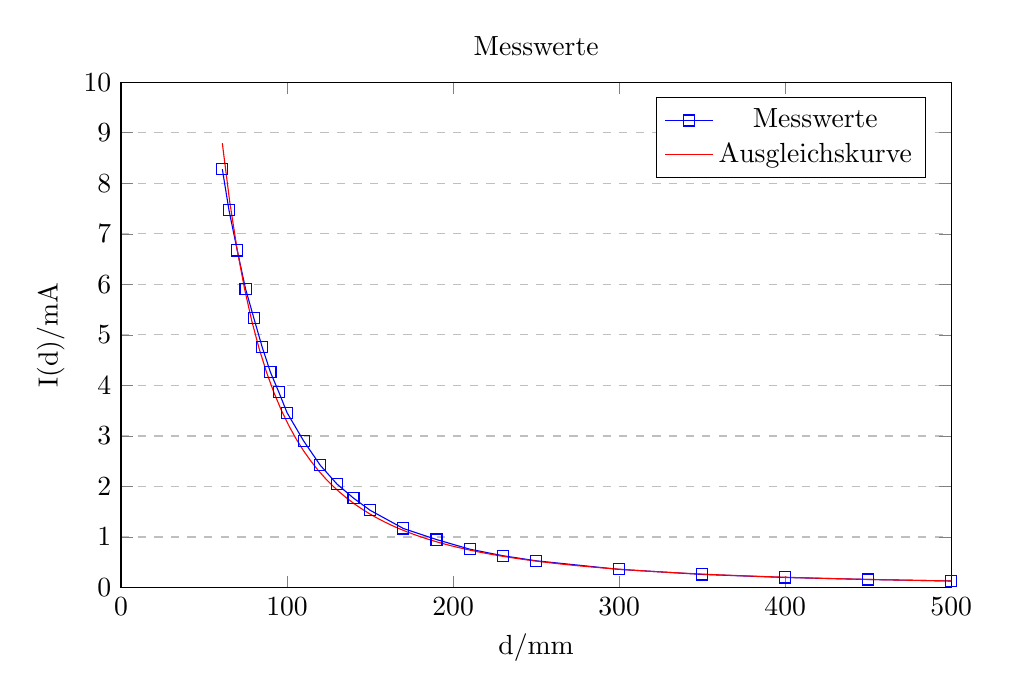
\begin{tikzpicture}
    \begin{axis}[
        title={Messwerte},
        xlabel={d/mm},
        ylabel={I(d)/mA},
        xmin=0, xmax=500,
        ymin=0, ymax=10,
        xtick={0,100,200,300,400,500},
        ytick={0,1,2,3,4,5,6,7,8,9,10},
        legend pos=north east,
        ymajorgrids=true,
        grid style=dashed,
    ]

    \addplot[
        color=blue,
        mark=square,
    ]
    coordinates {
        (61,8.28)(65,7.47)(70,6.67)(75,5.91)(80,5.33)(85,4.76)(90,4.26)(95,3.87)(100,3.46)(110,2.90)(120,2.42)(130,2.05)(140,1.77)(150,1.53)(170,1.17)(190,0.95)(210,0.76)(230,0.63)(250,0.53)(300,0.36)(350,0.26)(400,0.20)(450,0.16)(500,0.13)
    };
    \addlegendentry{Messwerte}

    \addplot [
        domain=61:500,
        samples=100,
        color=red,
    ]
    {(5.528491 * 10^(-3) * x)^(-2)};
    \addlegendentry{Ausgleichskurve}

    \end{axis}
\end{tikzpicture}

\textbf{Ausgleichskurve:} $y=(5.528491 * 10^{-3} * x)^{-2}$

\subsection{Statistik}

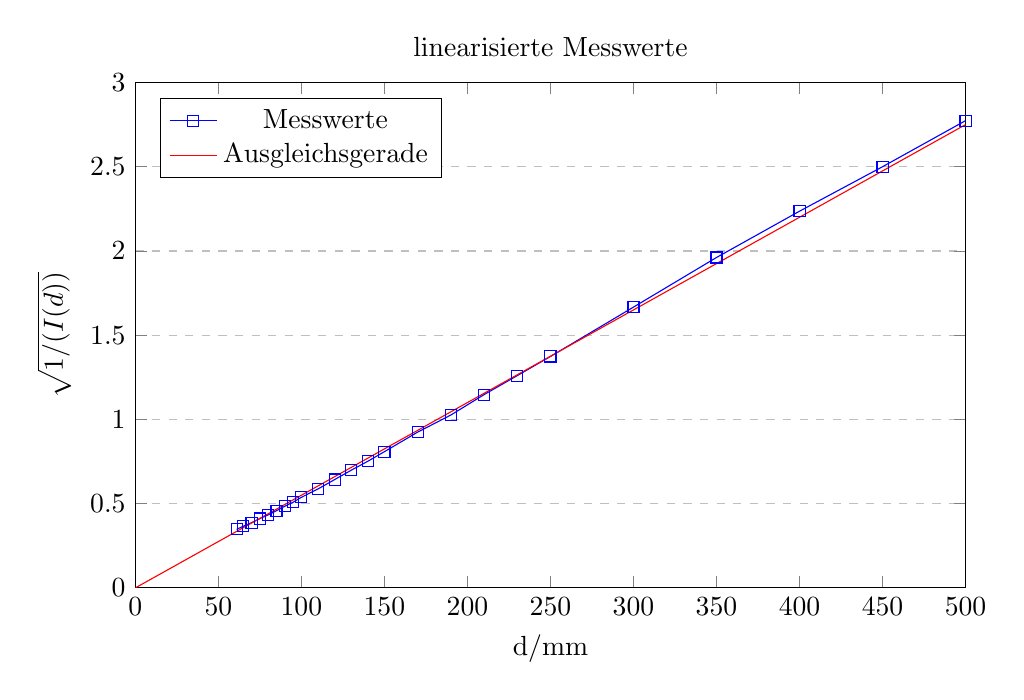
\begin{tikzpicture}
    \begin{axis}[
        title={linearisierte Messwerte},
        xlabel={d/mm},
        ylabel={$\sqrt{1/(I(d))}$},
        xmin=0, xmax=500,
        ymin=0, ymax=3,
        legend pos=north west,
        ymajorgrids=true,
        grid style=dashed,
    ]

    \addplot[
        color=blue,
        mark=square,
    ]
    coordinates {
        (61,0.34752402342845795)(65,0.3658808666323012)(70,0.38720154633118314)(75,0.41134503489486357)(80,0.43314808182420994)(85,0.45834924851410563)(90,0.4845015831115092)(95,0.5083285677753488)(100,0.5376033305704704)(110,0.5872202195147035)(120,0.6428243465332251)(130,0.6984302957695783)(140,0.7516460280028289)(150,0.8084520834544433)(170,0.9245003270420485)(190,1.025978352085154)(210,1.1470786693528088)(230,1.259881576697424)(250,1.37360563948689)(300,1.6666666666666667)(350,1.9611613513818402)(400,2.23606797749979)(450,2.5)(500,2.7735009811261455)
    };
    \addlegendentry{Messwerte}

    \addplot [
        domain=0:500,
        samples=100,
        color=red,
    ]
    {0.0055 * x};
    \addlegendentry{Ausgleichsgerade}

    \end{axis}
\end{tikzpicture}\\\\\\
\textbf{Linearisierung:} $y=\sqrt{1/(U(d))}$\\
\textbf{Ausgleichsgerade:} $y=0.0055x$\\
\textbf{Rücktransformation:} $y = 1/(0.0055x)^2 = 33057.9*x^-2$

\vspace{5mm}
Wie im Graphen und an der Ausgleichsgerade zu sehen verlaufen die Messwerte antiproportional. Um die Genauigkeit der Gerade zu analysieren berechnen wir eine Antiproportionalitätskonstante:

\vspace{10mm}

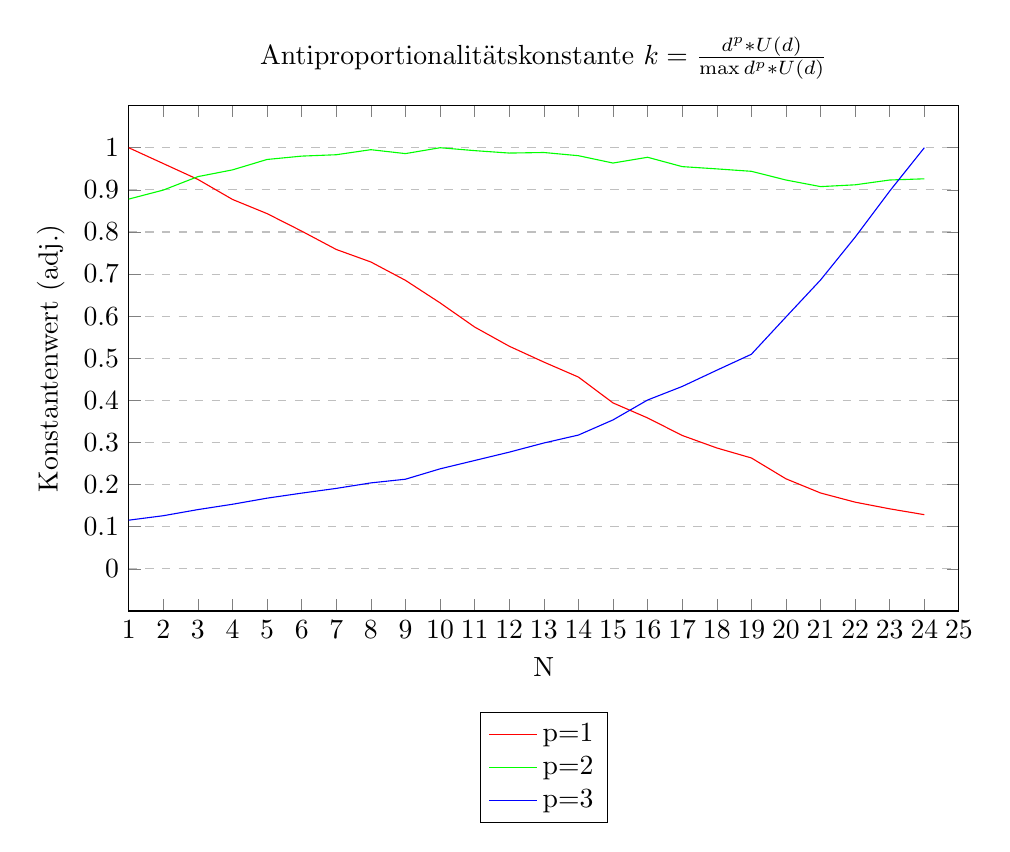
\begin{tikzpicture}
    \begin{axis}[
        title={Antiproportionalitätskonstante $k = \frac{d^p * U(d)}{\max{d^p * U(d)}}$},
        xlabel={N},
        ylabel={Konstantenwert (adj.)},
        xtick={1,2,3,4,5,6,7,8,9,10,11,12,13,14,15,16,17,18,19,20,21,22,23,24,25},
        ytick={0,0.1,0.2,0.3,0.4,0.5,0.6,0.7,0.8,0.9,1},
        xmin=1, xmax=25,
        ymin=-0.1, ymax=1.1,
        legend style={at={(0.5,-0.2)},anchor=north},
        ymajorgrids=true,
        grid style=dashed,
    ]

    \addplot[
        color=red,
    ]
    coordinates {
        (1,1)(2,0.9623762376237623)(3,0.9247524752475248)(4,0.8772277227722772)(5,0.8435643564356435)(6,0.801980198019802)(7,0.7584158415841584)(8,0.7287128712871287)(9,0.6851485148514852)(10,0.6316831683168317)(11,0.5742574257425742)(12,0.5287128712871287)(13,0.4910891089108911)(14,0.45544554455445546)(15,0.3940594059405941)(16,0.3584158415841584)(17,0.31683168316831684)(18,0.2871287128712871)(19,0.2633663366336634)(20,0.21386138613861386)(21,0.1801980198019802)(22,0.15841584158415842)(23,0.14257425742574256)(24,0.12871287128712872)
    };
    \addlegendentry{p=1}

    \addplot[
        color=green,
    ]
    coordinates {
        (1,0.878027928184668)(2,0.899430037047592)(3,0.9314049586776859)(4,0.947392419492733)(5,0.9721288116272442)(6,0.9800797948133372)(7,0.9833570817896836)(8,0.9953548019378741)(9,0.9860359076660017)(10,1)(11,0.993103448275862)(12,0.98731832430892)(13,0.988657737247079)(14,0.9810487318324309)(15,0.9636078654887432)(16,0.9773439726417783)(17,0.9551439156454831)(18,0.9497577657452265)(19,0.9440011399259048)(20,0.9233399829011114)(21,0.9076660017098889)(22,0.9119407238529496)(23,0.9233399829011114)(24,0.9261897976631519)
    };
    \addlegendentry{p=2}

    \addplot[
        color=blue,
    ]
    coordinates {
        (1,0.11565556923076924)(2,0.12624301538461538)(3,0.14078830769230768)(4,0.1534326769230769)(5,0.167936)(6,0.17989138461538462)(7,0.19111015384615385)(8,0.20418713846153846)(9,0.2129230769230769)(10,0.23753230769230768)(11,0.25733907692307695)(12,0.27716)(13,0.2988849230769231)(14,0.31776923076923075)(15,0.353736)(16,0.4009876923076923)(17,0.43312984615384614)(18,0.47170523076923077)(19,0.5096153846153846)(20,0.5981538461538461)(21,0.686)(22,0.7876923076923077)(23,0.8972307692307693)(24,1)
    };
    \addlegendentry{p=3}

    \end{axis}
\end{tikzpicture}

\vspace{10mm}

Deutlich zu sehen ist hier, dass der Graph für $p=2$ relativ konstant bleibt. Dies deutet auf eine Funktion $y=1/x^2$ hin.

\newpage

\subsection{Theorie}
\subsubsection{Das $1 / x^2$ Abstandsgesetz}
Bei einem punktförmigen Strahler (etwa der Halogenbirne, welche in diesem Experiment verwendet wurde) gilt das $1/r^2$-Abstandsgesetz.
Dieses sagt aus, dass sich die wahrgenommene Intensität beim Erhöhen des Abstands zum Strahler antiproportional zum Quadrat des Abstandes verändert.

Das Gesetz lässt sich einfach anhand des Strahlensatzes erklären:

\begin{figure}[h]
    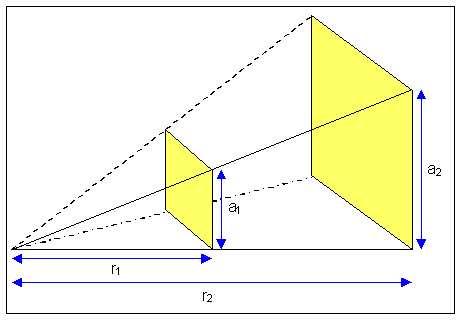
\includegraphics[width=\textwidth]{Strahlensatz.png} % Quelle: http://www.gsg-physik.net/physik/abstandsgesetz/strahlensatz.gif
    \caption[Strahlensatz]{Strahlensatz}
\end{figure}

Die punktförmige Quelle scheint auf zwei Ebenen. Für die Größe der Ebenen gilt:
$$r_2=2*r_1$$
$$a_1 / r_1 = a_2 / r_2$$
$$a_1 / r_1 * r_2 = a_2$$
$$a_1 / r_1 * (2 * r_1) = a_2$$
$$a_1 * r_1 = a_2$$
$$A_2 = a_2^2$$
Beim verdoppeln des Abstandes vervierfacht sich also die Fläche der Ebene (die Intensität pro Flächeneinheit viertelt sich):
$$a_2^2=2^2 * a_1^2 = 4 * a_1^2$$
Das Licht, welches vorher auf die kleinere Fläche geschienen hat, muss jetzt die gesamte, größere Fläche ausfüllen. Hierdurch verändert sich die Intensität pro Flächeneinheit also um $1/x^2$.

Durch die punktförmige, isotrope Ausgangsform des Lichtes lässt sich diese Annehmung vereinfachen:
Das Licht muss durch die kugelförmige Ausbreitung immer die Oberfläche der gesamten Kugel füllen. Da für die Kugeloberfläche $A=4*\pi*r^2$ gilt, sieht man hier, dass die Bestrahlungsstärke hier ebenfalls quadratisch antiproportional abnimmt:
$$1/A = 1/(4 * \pi * r^2) ~ 1/r^2$$

\subsection{Fazit / Reflexion}
Anhand des Graphen in $3.2$ lässt sich deutlich erkennen, dass die Messwerte der in $3.4.1$ genannten Theorie entsprechen.
Der hohe Maßkorrelationskoeffizient von $r = 0.9999$ bei der Annahme von $y=1/x^2$ bestätigt dies erneut. 

\end{document}
